\chapter{Implementation}\label{implementation}

\section{Persistenz}
\subsection{Auswahl Persistenz-Provider}
Bereits zu Beginn stellte sich die Frage, warum man welche der drei m\"oglichen und im Abschnitt ``\ref{grundlagen:persistenz} \titleref{grundlagen:persistenz}'' aufgelisteten Persistenz-Provider Mapper, Record oder ScalaJPA  verwenden sollte.

Ich versuchte herauszufinden und auszuf\"uhren, wie weit Ans\"atze hinsichtlich Dokumentation, aktive Weiterentwicklung und Reifegrad der Implementation sind.

\subsubsection{Aktive Weiterentwicklung}
Ein Blick auf die verschiedenen Commit Histories der Persistenz Module Mapper\footnote{http://github.com/lift/lift/commits/master/framework/lift-persistence/lift-mapper} und Record\footnote{http://github.com/lift/lift/commits/master/framework/lift-persistence/lift-record} zeigt schnell auf, dass in beiden Frameworks aktiv nicht sonderlich viel geschieht. \"Anderungen im Bereich der Persistenz-Libraries finden momentan vorallem im Bereich der NoSQL Datenbanken statt. 

\subsubsection{Dokumentation}
W\"ahrend die Dokumentation von Mapper\footnote{http://www.assembla.com/wiki/show/liftweb/Mapper} noch einigermassen anspricht, kann man zum Mapping mit dem Record Framework ausser ganz wenige Beispiele in \cite[p. 79 - 113]{chen2009lift} nicht viel auffinden.

\subsubsection{Reifegrad}
Der Reifegrad der im Lift Framework enthaltenen Persistenz-Bibliotheken ist meines Erachtens gering. Anforderungen wie das Mappen von Hierarchien (Beispiele in Hibernate Table per Klasse, Table per Hierarchie) fehlen g\"anzlich. Die Relationen zwischen den Klassen sind relativ unflexibel und gen\"ugen h\"ochstens, wenn man ein Projekt auf der ``Gr\"unen Wiese'' starten kann. Der dritte wichtige Mangel ist, dass mit der Verwendung von Mapper und Record eine Kopplung der gesamten Applikation ans Persistenz-Framework passiert. Siehe dazu Abschnitt ``\ref{persistenz:kopplung} \titleref{persistenz:kopplung}''.


\subsubsection{Fazit}
Meines Erachtens liefern Mapper und Record nicht das, was wir uns von bereits existierenden Frameworks wie Hibernate gewohnt sind. Ich habe mich aus oben beschriebenen Gr\"unden dazu entschieden, JPA 2.0 und Hibernate in der Version 3.5.1 im Persistenz-Layer zu verwenden. 

\subsection{Domain Mapping}
Ich habe die Mappings der Dom\"anenklassen mittels im Abschnitt ``\ref{grundlagen:integration:java} \titleref{grundlagen:integration:java}'' kurz angesprochenen Annotationen gemacht. Ich gehe im folgenden auf das Mapping der User Klasse ein, werde aber an dieser Stelle auf die Beschreibung der Mappings aller Klassen verzichten. 

\subsubsection{Klasse User}
Die Mapping Informationen f\"ur Hibernate respektive JPA befinden sich in Klasse ch.plannr.model.User. Die Klasse verwendet als Mixins folgende Traits:
\begin{itemize}
	\item \textbf{MegaBasicUser - } verf\"ugt in Anlehnung an MegaProtoUser\footnote{Mega ProtoUser ist die Basis-User-Klasse f\"ur das Mapper Framework und stellt eine Basis f\"ur die Benutzerverwaltung zur Verf\"ugung} \"uber die Funktionalit\"aten, die im Zusammenhang mit der Registrierung, Login, Passwort-Reset ben\"otigt werden. 
	\item \textbf{Domain -} definiert abstrakte Methoden zur Umwandlung von Objekten in XML und in die JSON\footnote{Javascript Object Notation}. 
	\item \textbf{Persistent - }Stellt in Anlehnung an das Active Record Design Pattern Methoden zum Persistieren, L\"oschen, Editieren von Objekten zur Verf\"ugung. Die Klasse Persistent verwendet f\"ur die beschriebenen Operationen eine ThreadLocal basierten EntityManager. Mit diesem Konstrukt wird die Thread-Safety dieses EntityManagers sicher gestellt und gleichzeitig ein lokaler Context f\"ur die Attachten Klassen definiert.	
\end{itemize}

Zu persistierende Objekte werden als Entities bezeichnet und m\"ussen in JPA mit 
\begin{lstlisting}[caption=User: ScalaJPA Entity Definiton]
@Entity
@Table(name = "TBL_USER")
\end{lstlisting}

annotiert werden. Mit Table kann man den Tabellennamen spezifizieren. Was auch ein Mapping auf Legacy Datenbanken erm\"oglichen w\"urde.

Die Id des Benutzers kann bei bestimmten Datenbanken automatisch ermittelt werden. In meinem Fall MySQL wird das mittels 
\begin{lstlisting}[caption=User: ScalaJPA Id mit Auto-Increment]
@Id
//@GeneratedValue(
//	strategy = GenerationType.SEQUENCE, 
//	generator="user_seq")
@GeneratedValue(strategy = GenerationType.AUTO)
@Column(name = "ID")
var id: Long = _
\end{lstlisting}
gemappt. Im Fall von Oracle m\"usste der GenerationType.SEQUENCE verwendet werden.
Normale Properties ben\"otigen eigentlich keine Annotation mehr, per Default werden in JPA alle Properties als Spalten angelegt, mit der @Column Annotation kann man allerdings die Defaults (Constraints, Spaltenname) \"uberschreiben. @NotNull und @NotEmpty sind Annotationen zur Validierung von Objekten (siehe Abschnitt ``\ref{jpa:validation} \titleref{jpa:validation}''). Die Annotation @BeanProperty sorg daf\"ur, dass f\"ur ein Feld Getter- und Setter-Methoden erstellt werden. Dies ist vorallem zur Interoperabilit\"at mit Java-Frameworks teilweise m\"oglich - in diesem Fall wird es ebenfalls f\"ur die Validierung ben\"otigt. 
\begin{lstlisting}[caption=User: ScalaJPA firstname Mapping]
@Column(name = "FIRST_NAME", nullable = false)
@NotNull
@NotEmpty
@BeanProperty
var firstname: String = _
\end{lstlisting}

Des weiteren sind die Annotationen @Embedded\footnote{@Embedded bietet die M\"oglichkeit, Attribute zwar in der selben Tabelle (embedded) zu speichern, allerdings im Objekt-Orientierten Modell in ein andere Instanz wie zum Beispiel in ein Adress-Objekt abzurufen} und die verschiedenen Beziehungen zu anderen Tabellen @ManyToOne, @OneToMany und @ManyToMany\footnote{Mittels @ManyToOne, @OneToMany, @ManyToMany k\"onnen uni- und bidirektionale Beziehungen realisiert werden.} interessant. 



\subsection{Validation}\label{jpa:validation}
Annotationen wie @NotNull, @Null, @Past, @Future sind definiert \"uber den JSR330 (Bean Validation 1.0). Mittels Bean Validation lassen sich Validierungen auf allen Ebenen des Systems durchf\"uhren. Zum Beispiel lassen sich User-Objekte bereits ohne Speicherung validieren und entsprechend f\"ur jedes Property Fehlermeldungen in der View bereitstellen. Auf der Ebene der Datenbank k\"onnen anhand dieser annotierten Properties automatisch Constraints  generiert werden.

Alle Dom\"anenklassen die als Mixin die bereits erw\"ahnte Klasse Persistent[T] verwenden k\"onnen mittels der methode validate validiert werden. Die Validierung wird vollumf\"anglich anhand der in den Klassen enthaltenen Annotationen gemacht. Als R\"uckgabewert werden die Constraints-Verletzungen innerhal eines Sets zur\"uckgeliefert. Ich verwende diese Constraints-Verletzungen weiter f\"ur die Anzeige in der View. Zum Beispiel der Validierung bei der Registrierung werden bei unvollst\"andiger Eingabe folgende Fehler angezeigt:
 \begin{figure}[H]
  	\centering
    	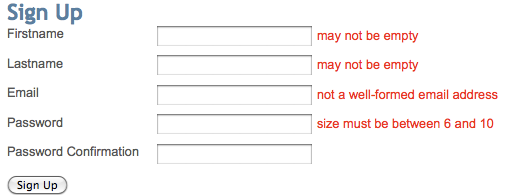
\includegraphics[width=12cm]{images/validation_registration}
        	\caption{Formular Validierung: Registration}
\end{figure}


Die Implementation der Methode validate ist relativ einfach und sieht folgendermassen aus:
\begin{lstlisting}[caption=Validation innerhalb der Klasse Persistence]
@Transient
private val validatorFactory = 
		Validation.buildDefaultValidatorFactory();

@Transient
private val validator = validatorFactory.getValidator();
  
def validate() = {
  validator.validate(this)
}
\end{lstlisting}
\section{Benutzermanagement}
Sofern man bei der Entwicklung von Webapplikationen mittels Lift den Persistenz-Provider Mapper ausw\"ahlt, erh\"alt man Benutzerverwaltung inklusive Login-, Registrierung- und Passwort-Reset-Mechanismus mitgeliefert und kann diesen relativ flexibel erweitern. Sofern man sich f\"ur JPA entscheidet, muss dies - insbesondere weil die Kopplung zwischen Dom\"anenklassen und Mapper respektive Record so hoch ist - selber implementieren. In anlehnung an ProtoUser, MegaProtoUser und MetaMegaProtoUser vom Mapper-Framework habe ich Funktionalit\"at \"ubernommen und MegaBasicUser respektive MetaMegaBasicUser f\"ur das Mapping mit JPA implementiert. In Sachen LOC\footnote{Lines of Code} haben die Klassen noch etwas Optimierungspotential, in Sachen Registrierung, Login, Validierung, Passwort Reset, Benutzer Editierung tun sie aber ihren Zweck. Als kurze Erl\"auterung die Beschreibung zur Funktionalit\"at f\"ur das Passwort-Reset beispielhaft:

\begin{lstlisting}[caption=Implementation Funktionalit\"at Passwort-Reset]
def passwordReset(id: String) =
    findById(id.toLong) match {
      case Full(user) =>
        def finishSet() {
          val violations = user.validate
          if (violations.size == 0)
            user.merge
          else {
            val node: NodeSeq = violations
            S.error(node)
            S.redirectTo("/")
          }
        }

        bind("user", HtmlTemplate.passwordResetXhtml,
          "pwd" -> 
            password_*("", (p: List[String]) =>
              user.password = p.head),
          "submit" -> 
            submit(S.??("set.password"), finishSet _))
      case _ => 
        S.error(S.??("password.link.invalid")); 
        S.redirectTo(homePage)
    }
\end{lstlisting}
Die Methode zum Reset des Passworts wird vom Menu respektive der Lift-Internen SiteMap Funktionalit\"at (siehe unter: ``\ref{lift:sitemap} \titleref{lift:sitemap}'') aufgerufen. Dies allerdings nur, wenn der Benutzer in der Http-Session angemeldet ist.  Der R\"uckgabewert der passwordReset-Methode ist ein Objekt vom Typ scala.xml.NodeSeq, welches das eigentliche Formular repr\"asentiert. Eingabefelder werden nicht in reinem HTML definiert, sondern via die Verwendung der Methoden text, password, usw. Diese Methoden der Klasse SHtml registrieren zum einen eine Callback-Funktion, zum anderen geben sie das auszugebenden Xml-Element als scala.xml.Elem zur\"uck. Beim \"Ubermitteln des Formulars wird dann die entsprechend zu einer definierten ID registrierte Callback-Funktion mit dem vom Benutzer eingegebenen Wert aufgerufen. Zum einen wird somit f\"ur die Textfelder der Wert hinterlegt, zum anderen via die Methode finishSet der Benutzer validiert und gespeichert. 

Alle Formulare der Benutzerverwaltung sind in etwa auf diese Weise implementiert. 

\section{Navigation}
Da die Ferienplanung und Administration der Benutzer vollumf\"anglich in Flex implementiert ist, basiert auch die Navigation dieser Beiden Use Cases auf Flex Komponenten wie Tab-Panels sowie States und Transitions (siehe: ``\ref{implementation:ferienplanung} \titleref{implementation:ferienplanung}'').  Ausserhalb ist die Navigation mittels der Lift-Sitemap implementiert. Wie bereits unter ``\ref{lift:sitemap} \titleref{lift:sitemap}'' angek\"undigt bezieht sich die Lift-Sitemap nicht nur auf das Verlinken von Seiten, sondern auch f\"ur die Zugriffskontrolle. Die Struktur des Menus sieht folgendermassen aus:

\begin{spacing}{0.5}
  \begin{longtable}{|p{2cm}|p{5cm}|p{6cm}|}
      \caption{Navigation und Menustruktur}\\
\hline
  \textbf{Name} & \textbf{Link} & \textbf{Constraints}\\
  \hline
  Home & /index & keine\\
  \hline
  Manager & /manager & Benutzer angemeldet\\
  \hline
  Login & /user\_mgt/login & Benutzer nicht angemeldet\\
  \hline
  Benutzer registrieren & /user\_mgt/sign\_up & Benutzer nicht angemeldet\\
  \hline
  Passwort verloren & /user\_mgt/lost\_password & Benutzer nicht angemeldet\\
  \hline
  Logout & /user\_mgt/logout & Benutzer angemeldet\\
  \hline
 Passworter reset & /user\_mgt/reset\_password & Benutzer angemeldet\\
  \hline
  Benutzer editieren & /user\_mgt/edit & Benutzer angemeldet\\
  \hline
  Passwort \"andern & /user\_mgt/change\_password & Benutzer angemeldet\\
  \hline
  \end{longtable}
\end{spacing}

Das Menu wird aus einer Liste von Menu-Eintr\"agen in der Klasse Boot.scala definiert und in die SiteMap gesetzt. Die Zugriffssteuerung wird \"uber die LocParams implementiert die sich in den Menu Instanzen befinden. 
 
\section{Flex Client}
F\"ur die Administration der Teams sowie auch f\"ur die Ferienplanung habe ich mich wegen von mir subjektiv empfundener besserer Usability und der M\"oglichkeit eines etwas besseren Software-Designs f\"ur Adobe Flex entschieden. 
\subsection{Software-Design}
Die meisten User-Interfaces zeichnen sich, insbesondere durch die hohe Kopplung zwischen Komponenten, durch eine extrem schlechte Wartbarkeit aus. Diese Problematik kann in Applikationen verschiedenster Frontend-Technologien auftreten - egal ob Javascript, Flex, GWT oder Silverlight. Eine weitere Schwierigkeit bei diesen Applikationen sind die angemessene und zentrale Behandlung von auftretenden Events, die Verf\"ugbarkeit von Contexten und die Unterst\"utzung in der Anbindung an Backend-Systemen. Damit solche Problemstellungen f\"ur diesen Client minimiert werden k\"onnen, habe ich eine kurze Evaluation bestehender Flex-Frameworks durchgef\"uhrt und dabei die folgenden angeschaut:
\begin{itemize}
\item \textbf{Cairngorm\cite{Cairngorm} - } unter Flex 2 und 3 war Cairngorm noch ein Frameworks mit Fokus auf die MVC-Architektur von Client-Applikationen. Mittlerweile handelt es sich allerdings um ein breiteres Set von Guidelines, Tools und Bibliotheken. Welche sich frameworkunabh\"angig einsetzen lassen. Mittlerweile basieren viele dieser Bibliotheken auf anderen Dependency Injection und MVC Frameworks wie Parsley, Swiz, oder Spring ActionScript
\item \textbf{Mate\cite{Mate} - } in erster Linie wurde Mate f\"ur das Event-Handling entwickelt. Die Art und Weise der Konfiguration findet deklarativ via ein MXML statt und ist relativ unflexibel:

\begin{lstlisting}[caption=Event-Deklaration mit dem Mate Framework]
<EventHandlers type="{MessageEvent.GET}">
  <RemoteObjectInvoker 
    instance="{services.helloService}" 
    method="sayHello" 
    arguments="{event.name}">
    <resultHandlers>
      <CallBack 
        method="handleResult" 
        arguments="{resultObject.text}"/>
    </resultHandlers>
    <faultHandlers>
      <CallBack 
        method="handleFault" 
        arguments="{fault.faultDetail}"/>
    </faultHandlers>
    </RemoteObjectInvoker>
</EventHandlers>
\end{lstlisting}

\item \textbf{Switz\cite{Swiz} - }ist meines Erachtens das flexibelste und am elegantesten zu konfigurierende Framework. Es stellt folgende drei Hauptfunktionalit\"aten zur Verf\"ugung:
\begin{itemize}
	\item \textbf{Dependency Injection} als Basis zur Inversion of Control anhand eines Beispieles. Beans und somit der applikationsweite Context werden in einer MXML-Datei definiert:
\begin{lstlisting}[caption=Swiz: Bean Deklaration]
<swiz:BeanProvider ...>
  <fx:Declarations>
    <core:Context id="context"/>
  </fx:Declarations>
</swiz:BeanProvider>
\end{lstlisting}

Objekte k\"onnen nun in beliebeigen MXML-Dateien oder ActionScript Klassen injected werden - selbst two-way Bindings sind m\"oglich:
\begin{lstlisting}[caption=Swiz: Bean Injection]
[Inject(source="context.selectedTeam", 
        bind="true",
        twoWay="true")]
public var selectedTeam:Team = null;
\end{lstlisting}
\item \textbf{Event Handling} zur entkopplung von Mediator und Observer. Events werden mit der Methode dispatchEvent(Event e) des Interfaces IEventDispatcher geworfen werden. MXML sind grunds\"atzlich von diesem Typ, in normalen ActionScript-Klassen kann ein entsprechender Dispatcher injected werden. Um sich f\"ur Events zu registrieren ist eine Methode mit folgender Signatur und Annotation zu implementieren:

\begin{lstlisting}[caption=Swiz: Event Observer]
[Mediate( event="Events.SEARCH_USERS", 
          properties="term" )]
public function searchUsers( term:String) : void
{
//...
}
\end{lstlisting}
Hier wird das Property term des geworfenen Events zus\"atzlich der Methode als Argument \"ubergeben.
\item Einfacher Lifecycle f\"ur asynchrone Aufrufe auf Remote Systeme.
\end{itemize}
\end{itemize}

Aufgrund der Einfachheit des Swiz-Frameworks, der Flexibilit\"at und der eleganten Konfiguration habe ich mich gegen Cairngorm und Mate entschieden und das Event-Handling sowie Context und Dependency Injection mit Swiz implementiert.

\subsection{Architektur}
Flex-Applikationen werden als Flash-Dateien dem Browser gesendet und laufen innerhalb der Flash Runtime Umgebung. Verglichen mit HTML 4.0.1 und XHTML 1.0 hat man mit Flex die M\"oglichkeit, Daten respektive Zust\"ande clientseitig zu Speichern. In der Praxis w\"are es auch m\"oglich, ganz auf den Browser zu verzichten - dann l\"asst man die Flex-Applikation in der Adobe Air Runtime laufen. Hier h\"atte k\"onnte man Daten sogar Clientseitig in eine SQLLight Datenbank speichern. 

In meinem Fall wird der Flex-Client innerhalb der Lift-Applikation eingebettet und kommuniziert mit dem Backend via RESTful\cite{wiki:rest} Webservices. Siehe Abschnitt \ref{implementation:restful-webservices} \titleref{implementation:restful-webservices}. Hinsichtlich eines einfacheren Implementationsaufwandes w\"are es Sinnvoll, ob ein Framework zur Kommunikation wie BlazeDS\cite{blazeDs}\cite{IntegratingBlazeDsLiftweb} oder GranitDS\cite{graniteDs} nicht sinnvoll w\"are. F\"ur Informationen zum Thema Security siehe Abschnitt \ref{flex:security}.


\subsubsection{RESTful Webservices}\label{implementation:restful-webservices}
Nebest verschiedenen Konzepten wie die ``Betrachtung von Daten als Ressourcen'' ist die Verwendung der verschiedenen Http-Methoden POST, PUT, GET, DELETE, etc. 
Die Kommunikation von Flex-Applikationen zu anderen Systemen findet \"uber den darunterliegenden Browser statt, welcher in den meisten F\"allen PUT und DELETE nicht unterst\"utzt. Ein M\"oglicher Workaround f\"ur dieses Problem ist die Verwendung eines Http-Attributes wie zum Beispiel ''X-HTTP-Method-Override''. Bei PUT- und DELETE-Aufrufen setze ich dieses Attribut in den Http-Header (Beispiel: X-HTTP-Method-Override=PUT). Auf der Serverseite wird der eintretende Request gewrappt und Aufrufe wie request.getMethode() liefern anhand des Headers auch PUT oder DELETE zur\"uck. F\"ur weitere Informationen siehe
\begin{itemize}
\item Klasse ch.plannr.common.http.WrappedRequest.java,
\item Klasse ch.plannr.common.http.RequestWrapperFilter.scala,
\item web.xml
\end{itemize}
Auf Client-Seite wird das Attribute in der ActionScript-Klasse ch.plannr.service.HttpServiceFactory gesetzt. 

REST definiert grunds\"atzlich nicht, in welcher Form daten \"ubertragen werden m\"ussen. Es hat sich bereits etabliert, dass entweder Daten im XML- oder JSON-Format ausgetauscht werden. Aufgrund der XML-Unterst\"utzung in Scala (XML-Datentyp, Pattern-Matching auf XML) habe ich mich f\"ur XML entschieden.

\subsubsection{Security}\label{flex:security}
Zu Beginn habe ich die Authentifizierung der Webservice-Aufrufe \"uber Basic Authentication gemacht. Dies hat in der Praxis den wesentlichen Nachteil, dass prinzipiell alle Aufrufe verschl\"usselt werden m\"ussten. Basic Authentication \"ubermittelt das Passwort zwar nicht klartext, allerdings nur Base-64 Encoded. Somit k\"onnte man mit einem Sniffern sofort daran gelangen.
Nun habe ich die Authentifizierung auf eine Form-Authentication umgestellt, bei der die Benutzer-Identifikation respektive in meinem Fall die Email-Adresse in der Session gespeichert wird. Somit muss nur der Login-Formular Submit via das Https-Protokoll laufen.


\subsection{Ferienplanung}\label{implementation:ferienplanung}



\subsection{Teammanagement}\label{implementation:teammanagement}

\section{Mail-Versand (Notifikationen)}
\subsection{Use Cases}
Zu unterschiedlichen Zwecken m\"ussen  Emails an die Benutzer versendet werden. Die Email-Adressen gelten systemweit als Benutzer Identifikatoren und werden hierf\"ur auch verwendet. Nachfolgend eine Liste der Aktionen die einen Email-Versand zur Folge haben. Zus\"atzlich auch der Status der Implementation:
  \begin{longtable}{|p{3cm}|p{7cm}|p{3cm}|}
      \caption{Use Cases Email Versand}\\
\hline
  \textbf{Aktion} & \textbf{Beschreibung} & \textbf{Status der Implementation}\\
  \hline
  Signup&Nach der Registrierung wird zur Email-Validierung ein Email inklusive einem Link an den Benutzer versendet, \"uber welchen er den Account aktivieren kann. Im Link enthalten ist eine Zufallszahl so dass kein Missbrauch betrieben werden kann. & Nicht implementiert\\
  \hline
  Passwort vergessen&Sofern das Passwort vergessen geht, wird ein Email an den Benutzer versendet. \"Uber dieses Email kann das Passwort neu gesetzt werden. & Implementiert\\
  \hline
  Erfassung von Ferien durch den Mitarbeiter & Nachdem der Benutzer seine Ferienw\"unsche erfasst hat, geht ein Email an den Vorgesetzten, damit dieser die Eintr\"age \"uberpr\"ufen kann & Nicht implementiert \\
  \hline
  Status\"anderung durch Vorgesetzten & Nachdem der Vorgesetzte die Ferien \"uberpr\"uft und bewilligt, abgelehnt hat, wird der Mitarbeiter informiert & Nicht implementiert\\
  \hline
\end{longtable}
 
 \subsection{Technische Umsetzung}
 \subsubsection{Konfiguration des Mailers}
 In meinem Fall l\"asst sich der Lift-Mail-Support, der sich innerhalb der Klasse net.liftweb.util.Mailer befindet, nicht nur \"uber die definition der Properties (mail.smtp.host, mail.username, mail.password) konfigurieren - ich muss zus\"atzlich den Authenticator (Mailer.authenticator) des Objekts Mailer setzen.

 \subsubsection{Mails versenden}
  Mails k\"onnen nun mit dem Aufruf der folgenden Methode versendet werden:
\begin{lstlisting}[caption=]
    Mailer.sendMail(From(emailFrom), 
                    Subject(signupMailSubject),
                    (To(user.email) :: 
                    xmlToMailBodyType(msgXml) ::
                    (bccEmail.toList.map(BCC(_)))): _*)
\end{lstlisting} 

Das erste Argument ist die Absender-Adresse, das zweite das Subject und das dritte eine Liste bestehend aus Empf\"anger, Carbon Copy (CC), Blind Carbon Copy (BCC) und Mailbodies (HTML, Plain Text). Die Liste wird vom Lift Framework beim Verwenden wieder in ihre Bestandteile aufgel\"ost und mit Empf\"anger und Subject versendet. 

\chapter{Entwicklung, Build und Deployment}

\section{Build-System}Maven als Build-System basiert ebenfalls auf einem Plugin-Konzept und unterst\"utzt in den verschiedensten Bereichen des Build-Managements. Nicht zuletzt dank dem Grundsatz ``Convention over Configuration'' l\"asst es sich auf allen Plattformen im Nu deployen. Maven \"ubernimmt bei diesem Projekt eine vielzahl an Funktionen:

\begin{itemize}
\item \textbf{Dependency Management: } Maven l\"adt die im pom.xml definierten Abh\"angigkeiten von \"offentlichen Repositories. 
\item \textbf{Support Entwicklungsumgebung:  } Die grosse Verbreitung von Maven hat dazu gef\"uhrt, dass Entwicklungsumgebungen Adapter oder Plugins daf\"ur entwickelt haben vomit sich solche Projekte automatisch innerhalb der IDE konfigurieren. Dazu geh\"ort das Hinzuf\"ugen von Abh\"angigkeiten in den Source- und Build-Pfad, das korrekte setzen von Ausgabe-Ordner. 
\item \textbf{Clean, Compile, Package: }Der gesamte Build-Prozess f\"urs Test-System findet mit Maven statt. Bei der Entwicklung werden die Klassen allerdings von der Entwicklungsumgebung kompilliert - diese beschriebenen Targets sind deshalb da nicht n\"otig. 
\item \textbf{Profil Management - } Maven ist von Grund auf f\"ahig, verschiedene Profile zu definieren. Profile kann man beispielsweise dann verwenden, wenn Applikationen f\"ur Entwicklung, Test, Produktion in unterschiedlichen Umgebungen laufen. Dann gilt es meistens, unterschiedliche Konfigurationen zu verwenden. Profile brauche ich um folgende Probleme zu l\"osen:\begin{itemize}
\item Der Datenbank-Zugriff wird in der Entwicklungsumgebung direkt \"uber JDBC gemacht, in der Testumgebung auf der Stax-Cloud wird eine von Servern verf\"ugbare Datasource verwendet.
\end{itemize}
\end{itemize}
\section{Entwicklungsumgebung}
W\"ahrend der Entwicklung hilft Maven vorallem im Bereich des Dependency Managements - Abh\"angigkeiten werden automatisch geladen, das Projekt kann nach der \"Offnung sofort kompiliert und gestartet werden. Die meisten Funktionalit\"aten im Backend habe ich Test-Driven mit Scala-Specs entwickelt, ohne dass ich die Funktionalit\"at jedesmal im Browser nachvollzog. Tests kann man auf verschiedene Arten ausf\"uhren:
\begin{itemize}
\item Maven per Default unterst\"utzt die Ausf\"uhrung von JUnit-Tests, mit Plugins k\"onnen allerdings auch Scala-Specs oder andere Tests ausf\"uhren.
\item Entwicklungsumgebungen welche Scala unterst\"utzen, bringen meistens auch Funktionalit\"at zum Testen (Ausf\"uhrung von Scala Specs oder Scala Unit  Tests). 
\item Die Scala-Gemeinde richtet sich mehr und mehr auf das Simple Build Tool\cite{SimpleBuildTool} aus. Es handelt sich dabei um ein Tool welches ebenfalls Dependency Management, Test, Build, usw. unterst\"utzt und sich gegebenenfalls auch mit Maven kombinieren l\"asst. Bei der Entwicklung hat das Tool mir geholfen, die Tests auszuf\"uhren, indem es kontinuierlich auf \"Anderungen wartet, neu Kompiliert und entsprechend die Tests neu ausf\"uhrt. Das somit schnelle Feedback kann den Entwicklungsprozess massiv beschleunigen.\end{itemize}


\section{Test- und Produktiv-Umgebung}
Um die Applikation auch der Breiten Masse verf\"ugbar zu machen, habe ich sie auf der Cloud-Plattform namens Stax\cite{Stax} deployt. Bei der Verfolgung von Twitter-Nachrichten verschiedener Personen und Diensten bin ich auf diese Plattform aufmerksam geworden und die Einfachheit des Deployments hat mich sehr \"uberrascht.

F\"ur das Deployment auf diese Plattform musste ich folgende \"Anderungen durchf\"uhren:
\begin{itemize}
\item \textbf{Stax-Konfiguration f\"ur Maven - } F\"ur Maven ist ein Stax-Plugin vorhanden, das mittels der folgenden Zeilen im pom.xml konfiguriert werden muss: 

\begin{lstlisting}[caption=Konfiguration Maven mit Stax]
<build>
  <plugins>
    <plugin>
      <groupId>net.stax</groupId>
      <artifactId>stax-maven-plugin</artifactId>
    </plugin>
  ...
  </plugins>
</build>
\end{lstlisting}
Schlussendlich ist es m\"oglich, die Applikation mittels dem folgenden Kommando zu deployen:
\begin{lstlisting}[caption=Befehl Deployment Stax]
mvn clean stax:deploy -Pprod -Dstax.appid=plannr
\end{lstlisting}
\item \textbf{Stax-Konfiguration des Web Archives - } Wars f\"ur die Stax Plattform m\"ussen ein zus\"atzliches Xml mit dem namen stax-web.xml beinhalten. 
\item \textbf{Datasource Anbindung - } Via das Web-Interface von Stax kann eine neue MySql Datenbank auf der Cloud angelegt werden. Um der Applikation den Zugriff auf diese Datenbank zu erm\"oglichen, wird diese einerseits im stax-web.xml als auch im web.xml definiert. Die Aufl\"osung der Datasource wird zur Laufzeit \"uber den JNDI-Namen gemacht, der im persistence.xml definiert ist.
\item \textbf{Konfiguration JPA -} Damit sich der Persistenz-Provider nicht wie w\"ahrend der Entwicklungszeit direkt \"uber JDBC mit Url, Benutzernamen und Passwort verbindet, wird im Profilabh\"angigen persistence.xml f\"ur Test- und Produktiv-Umgebung die im web.xml als Ressource definierte Datasource verwendet. 
\end{itemize} 

Der Pfad f\"ur diese Dateien werden nur mit der Aktivierung \"uber das Maven-Profil geladen und \"uberschreiben die bereits bestehenden.







